% !TEX root=formulas-calculo.tex
% Author: Alfredo Sánchez Alberca (asalber@ceu.es)

\sloppy

\section*{Fórmulas de Cálculo}

\footnotesize
\tcbset{enhanced, colback=color1!10, colframe=color1, fonttitle=\bfseries\large\sffamily, %lifted shadow={1mm}{-2mm}{3mm}{0.1mm}
}

\begin{multicols}{2}
\subsection*{Geometría Analítica}

\begin{tcolorbox}[hbox, title=Vectores]
\begin{minipage}{0.4\textwidth}
\flushleft
\rule{0.4\textwidth}{0pt}
\begin{description}
\item[Vector que une dos puntos] $P=(p_1,\ldots,p_n)$, $Q=(q_1,\ldots,q_n)\in \mathbb{R}^n$
      \[
      \vec{PQ} = Q-P = (q_1-p_1,\ldots,q_n-p_n)
      \]
\item[Producto escalar] $\mathbf{u}=(u_1,\cdots,u_n)$, $\mathbf{v}=(v_1,\cdots,v_n)\in\mathbb{R}^n$
      \[
      \mathbf{u}\cdot \mathbf{v} = u_1v_1 + \ldots + u_nv_n
      \]
\item[Vectores ortogonales] (perpendiculares)
      \[
      \mathbf{u\cdot v}=0
      \]
\end{description}
\end{minipage}
\end{tcolorbox}

\begin{tcolorbox}[hbox, title=Rectas]
\begin{minipage}{0.4\textwidth}
\flushleft
\begin{description}
\item[Ecuación vectorial] de una recta que pasa por el punto $P$ con dirección del vector $\mathbf{v}$
      \[
      P+t\mathbf{v}
      \]
\item[Ecuación punto-pendiente] de una recta en $\mathbb{R}^2$ que pasa por el punto $(x_0,y_0)$ con pendiente $m$
      \[
      y=y_0+m(x-x_0)
      \]
\end{description}
\end{minipage}
\end{tcolorbox}

\begin{tcolorbox}[hbox, title=Planos]
\begin{minipage}{0.4\textwidth}
\begin{description}
\item[Ecuación general] de un plano en $\mathbb{R}^3$ que pasa por el punto $(x_0,y_0,z_0)$ perpendicular al vector $(a,b,c)$
      \[
      a(x-x_0)+b(y-y_0)+c(z-z_0)=0
      \]
\end{description}
\end{minipage}
\end{tcolorbox}


\subsection*{Trigonometría}

\begin{tcolorbox}[hbox, title=Triángulos rectángulos]
\begin{minipage}{0.4\textwidth}
\flushleft
\rule{0.4\textwidth}{0pt}
\begin{center}
\begin{tikzpicture}[
my angle/.style={
every pic quotes/.append style={text=cyan},
draw=cyan,
angle radius=1cm,
}]
\coordinate (C) at (-1.5,-1);
\coordinate (A) at (1.5,-1);
\coordinate (B) at (1.5,1);
\draw (C) -- node[above] {$h$} (B) -- node[right] {$o$} (A) -- node[below] {$a$} (C);
\draw (A) +(-.25,0) |- +(0,.25);
\pic [draw=cyan, angle radius=1cm, "$\theta$"] {angle=A--C--B};
\end{tikzpicture}
\end{center}
\begin{description}
\item[Seno] $\sen(\theta)=\dfrac{o}{h}$.
\item[Coseno] $\cos(\theta)=\dfrac{a}{h}$.
\item[Tangente] $\tg(\theta)=\dfrac{o}{a}=\dfrac{\sin(\theta)}{\cos(\theta)}$.
\item[Secante] $\sec(\theta)=\dfrac{h}{a}=\dfrac{1}{\cos(\theta)}$.
\item[Cosecante] $\cosec(\theta)=\dfrac{h}{o}=\dfrac{1}{\sen(\theta)}$.
\item[Cotangente] $\ctg(\theta)=\dfrac{a}{o}=\dfrac{\cos(\theta)}{\sen(\theta)}=\dfrac{1}{\tg(\theta)}$.
\end{description}
\end{minipage}
\end{tcolorbox}

\begin{tcolorbox}[hbox, title=Círculo unitario]
\begin{minipage}{0.4\textwidth}
\resizebox{\textwidth}{!}{
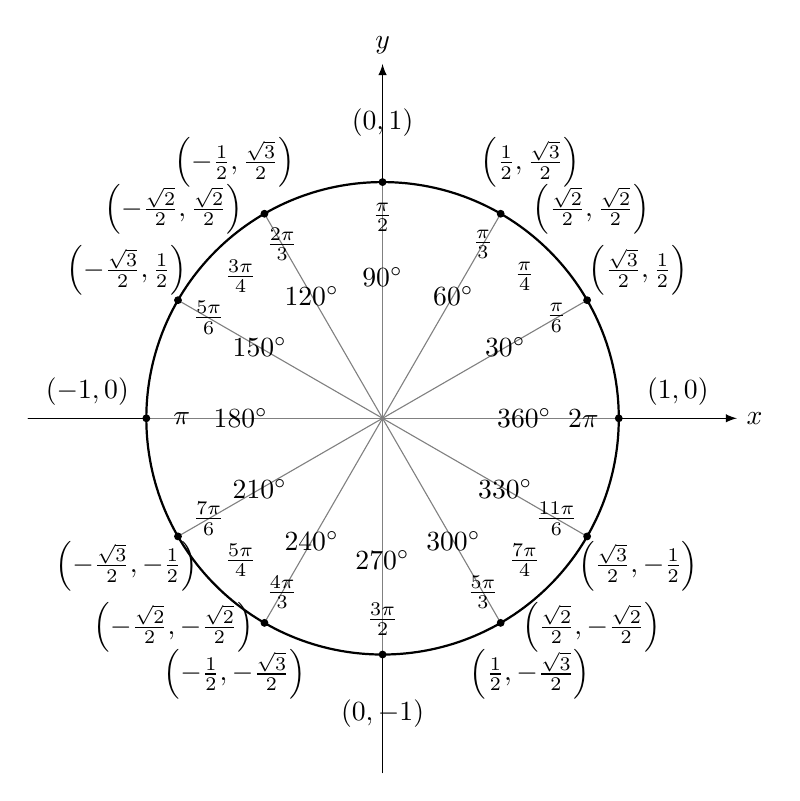
\begin{tikzpicture}[scale=3, cap=round, >=latex]
% draw the coordinates
\draw[->] (-1.5cm,0cm) -- (1.5cm,0cm) node[right] {$x$};
\draw[->] (0cm,-1.5cm) -- (0cm,1.5cm) node[above] {$y$};

% draw the unit circle
\draw[thick] (0cm,0cm) circle(1cm);

\foreach \x in {30,60,...,360} {
% lines from center to point
\draw[gray] (0cm,0cm) -- (\x:1cm);
% dots at each point
\filldraw[black] (\x:1cm) circle(0.4pt);
% draw each angle in degrees
\draw (\x:0.6cm) node[] {$\x^\circ$};
}

% draw each angle in radians
\foreach \x/\xtext in {
30/\frac{\pi}{6},
45/\frac{\pi}{4},
60/\frac{\pi}{3},
90/\frac{\pi}{2},
120/\frac{2\pi}{3},
135/\frac{3\pi}{4},
150/\frac{5\pi}{6},
180/\pi,
210/\frac{7\pi}{6},
225/\frac{5\pi}{4},
240/\frac{4\pi}{3},
270/\frac{3\pi}{2},
300/\frac{5\pi}{3},
315/\frac{7\pi}{4},
330/\frac{11\pi}{6},
360/2\pi}
\draw (\x:0.85cm) node[] {$\xtext$};

\foreach \x/\xtext/\y in {
% the coordinates for the first quadrant
30/\frac{\sqrt{3}}{2}/\frac{1}{2},
45/\frac{\sqrt{2}}{2}/\frac{\sqrt{2}}{2},
60/\frac{1}{2}/\frac{\sqrt{3}}{2},
% the coordinates for the second quadrant
150/-\frac{\sqrt{3}}{2}/\frac{1}{2},
135/-\frac{\sqrt{2}}{2}/\frac{\sqrt{2}}{2},
120/-\frac{1}{2}/\frac{\sqrt{3}}{2},
% the coordinates for the third quadrant
210/-\frac{\sqrt{3}}{2}/-\frac{1}{2},
225/-\frac{\sqrt{2}}{2}/-\frac{\sqrt{2}}{2},
240/-\frac{1}{2}/-\frac{\sqrt{3}}{2},
% the coordinates for the fourth quadrant
330/\frac{\sqrt{3}}{2}/-\frac{1}{2},
315/\frac{\sqrt{2}}{2}/-\frac{\sqrt{2}}{2},
300/\frac{1}{2}/-\frac{\sqrt{3}}{2}}
\draw (\x:1.25cm) node[] {$\left(\xtext,\y\right)$};

% draw the horizontal and vertical coordinates
% the placement is better this way
\draw (-1.25cm,0cm) node[above=1pt] {$(-1,0)$}
(1.25cm,0cm)  node[above=1pt] {$(1,0)$}
(0cm,-1.25cm) node[] {$(0,-1)$}
(0cm,1.25cm)  node[] {$(0,1)$};
\end{tikzpicture}
}
\end{minipage}
\end{tcolorbox}

\begin{tcolorbox}[hbox, title=Conversión de ángulos]
\begin{minipage}{0.4\textwidth}
\begin{description}
\item[Grados a radianes] $y=\dfrac{\pi \mbox{rad}}{180^\circ}x$.
\item[Radianes a grados] $y=\dfrac{180^\circ}{\pi \mbox{rad}}x$.
\end{description}
\end{minipage}
\end{tcolorbox}

\begin{tcolorbox}[hbox, title=Identidades pitagóricas]
\begin{minipage}{0.4\textwidth}
\[
\renewcommand{\arraystretch}{1.5}
\begin{array}{c}
\sen(\theta)^2 + \cos(\theta)^2 = 1 \\
1+\tg(\theta)^2 = \sec(\theta)^2    \\
1+\ctg(\theta)^2 = \cosec(\theta)^2
\end{array}
\]
\end{minipage}
\end{tcolorbox}

\begin{tcolorbox}[hbox, title=Razones trigonométicas de sumas de ángulos]
\begin{minipage}{0.4\textwidth}
\[
\renewcommand{\arraystretch}{1.5}
\begin{array}{c}
\sen{\alpha+\beta}=\sen(\alpha)\cos(\beta)+\cos(\alpha)\sen(\beta) \\
\sen{\alpha-\beta}=\sen(\alpha)\cos(\beta)-\cos(\alpha)\sen(\beta) \\
\cos{\alpha+\beta}=\cos(\alpha)\cos(\beta)-\sen(\alpha)\sen(\beta) \\
\cos{\alpha-\beta}=\cos(\alpha)\cos(\beta)+\sen(\alpha)\sen(\beta)\\
\sen(2\theta)=2\sen(\theta)\cos(\theta)\\
\cos(2\theta)=\cos(\theta)^2-\sen(\theta)^2
\end{array}
\]
\end{minipage}
\end{tcolorbox}


\subsection*{Derivadas de funciones de una variable}

\begin{tcolorbox}[hbox, title=Concepto de derivada]
\begin{minipage}{0.4\textwidth}
\flushleft
\rule{0.4\textwidth}{0pt}
\begin{description}
\item[Tasa de variación media] de una función $f(x)$ en un intervalo $[a,a+\Delta x]$
      \[
      \mbox{ARC}f[a,a+\Delta x] = \frac{\Delta y}{\Delta x} = \frac{f(a+\Delta x)-f(a)}{\Delta x}
      \]
\item[Tasa de variación instantánea (derivada)] de una función $f(x)$ en el punto $x=a$
      \[
      f'(a)=\lim_{\Delta x\rightarrow 0} \frac{\Delta y}{\Delta x} = \lim_{\Delta x\rightarrow 0}\frac{f(a+\Delta x)-f(a)}{\Delta x}
      \]
\end{description}
\end{minipage}
\end{tcolorbox}

\begin{tcolorbox}[hbox, title=Álgebra de derivadas]
\begin{minipage}{0.4\textwidth}
\flushleft
\rule{0.4\textwidth}{0pt}
\begin{description}
\item[Suma] $(u+v)'=u'+v'$
\item[Resta] $(u-v)'=u'-v'$
\item[Producto] $(u\cdot v)'=u'\cdot v+ u\cdot v'$
\item[Cociente] $\left(\dfrac{u}{v}\right)'=\dfrac{u'\cdot v-u\cdot v'}{v^2}$
\item[Regla de la cadena] $(f\circ g)'(x)=f'(g(x))g'(x)$
\end{description}
\end{minipage}
\end{tcolorbox}

\begin{tcolorbox}[hbox, title=Rectas secante y tangente]
\begin{minipage}{0.4\textwidth}
\flushleft
\begin{description}
\item[Recta secante] a la gráfica de $f(x)$ en los puntos $(a,f(a))$ y $(a+\Delta x, f(a+\Delta x))$
      \[
      y=f(a)+\mbox{ARC}f[a,a+\Delta x](x-a)
      \]
\item[Recta tangente] a la gráfica de $f(x)$ en el punto $(a,f(a))$
      \[
      y=f(a)+f'(a)(x-a)
      \]
\end{description}
\end{minipage}
\end{tcolorbox}

\begin{tcolorbox}[hbox, title={Crecimiento, concavidad y extremos}]
\begin{minipage}{0.4\textwidth}
\flushleft
\begin{description}
\item[Crecimiento]
      \begin{itemize}
      \item[]
      \item $\forall x\in I\ f'(x)\geq 0$ $\Rightarrow$ $f$ es creciente en $I$.
      \item $\forall x\in I\ f'(x)\leq 0$ $\Rightarrow$ $f$ es decreciente en $I$.
      \end{itemize}
\item[Concavidad]
      \begin{itemize}
      \item[]
      \item $\forall x\in I\ f''(x)\geq 0$ $\Rightarrow$ $f$ es cóncava hacia arriba en $I$.
      \item $\forall x\in I\ f''(x)\leq 0$ $\Rightarrow$ $f$ es cóncava hacia abajo en $I$.
      \end{itemize}
\item[Extremos] Si $f'(a)=0$ (punto crítico)
      \begin{itemize}
      \item $f''(a)<0$ $\Rightarrow$ $f$ tiene un máximo local en $x=a$.
      \item $f''(a)>0$ $\Rightarrow$ $f$ tiene un mínimo local en $x=a$.
      \end{itemize}
\end{description}
\end{minipage}
\end{tcolorbox}

\begin{tcolorbox}[hbox, title=Aproximación de funciones]
\begin{minipage}{0.4\textwidth}
\flushleft
\begin{description}
\item[Variación de una función]
      \[
      \Delta y\approx f'(a)\Delta x
      \]
\item[Polinomio de Taylor] de orden $n$ de $f(x)$ en el punto $x=a$
      \[
      P^n_{f,a}(x)=f(a)+f'(a)(x-a)+\frac{f''(a)}{2}(x-a)^2+\cdots+\frac{f^n(a)}{n!}(x-a)^n
      \]
\item[Polinomio de Maclaurin] de orden $n$ of $f(x)$
      \[
      P^n_{f,0}(x)=f(0)+f'(0)x+\frac{f''(0)}{2}x^2+\cdots+\frac{f^n(0)}{n!}x^n
      \]
\end{description}
\end{minipage}
\end{tcolorbox}



\subsection*{Ecuaciones diferenciales}

\begin{tcolorbox}[hbox, title=Ecuación diferencial de primer orden]
\begin{minipage}{0.4\textwidth}
\flushleft
\begin{description}
\item[Ecuación diferencial de primer orden]
      \[
      F(x,y,y')=0
      \]
\item[Problema del valor inicial]
      \[
      \left\{
      \begin{array}{ll}
      F(x,y,y')=0, & \hbox{EDO de primer orden;} \\
      y(x_0)=y_0,  & \hbox{Condición inicial.}   \\
      \end{array}
      \right.
      \]
\end{description}
\end{minipage}
\end{tcolorbox}

\begin{tcolorbox}[hbox, title=Resolución de EDO de primer orden]
\begin{minipage}{0.4\textwidth}
\flushleft
\begin{description}
\item[EDO de variables separables]
      \[
      y'g(y)=f(x)
      \]
      Solución:
      \[
      \int g(y)\,dy = \int f(x)\,dx+C.
      \]
\item[EDO lineal]
      \[
      y'+g(x)y = h(x)
      \]
      Solución:
      \[
      y=e^{-\int g(x)\,dx}\left(\int h(x)e^{\int g(x)\,dx}\,dx+C\right).
      \]
\end{description}
\end{minipage}
\end{tcolorbox}



\subsection*{Derivadas de funciones vectoriales}

\begin{tcolorbox}[hbox, title=Derivada de una función vectorial]
\begin{minipage}{0.4\textwidth}
\flushleft
Si $f(t)=(x_1(t),\ldots, x_n(t))$ entonces
\[
f'(t)=(x_1'(t),\ldots, x_n'(t))
\]
\end{minipage}
\end{tcolorbox}

\begin{tcolorbox}[hbox, title=Rectas tangente y normal en el plano]
\begin{minipage}{0.4\textwidth}
\flushleft
\begin{description}
\item[Recta tangente a una trayectoria en el plano] \mbox{$f(t)=(x(t),y(t))$} en el instante $t=a$
      \[
      \begin{array}{c}
      (x(a),y(a))+t(x'(a),y'(a)) \mbox{ o } \\
      (x-x(a))y'(a)-(y-y(a))x'(a)=0
      \end{array}
      \]
\item[Recta normal a una trayectoria en el plano] \mbox{$f(t)=(x(t),y(t))$} en el instante $t=a$
      \[
      \begin{array}{c}
      (x(a),y(a))+t(y'(a),-x'(a)) \mbox{ o } \\
      (x-x(a))x'(a)+(y-y(a))y'(a)=0
      \end{array}
      \]
\end{description}
\end{minipage}
\end{tcolorbox}

\begin{tcolorbox}[hbox, title=Recta tangente y plano normal en el espacio]
\begin{minipage}{0.4\textwidth}
\flushleft
\begin{description}
\item[Recta tangente a una trayectoria en el espacio] \mbox{$f(t)=(x(t),y(t),z(t))$} en el instante $t=a$
      \[
      (x(a),y(a),z(a))+t(x'(a),y'(a),z'(a))
      \]
\item[Plano normal a una trayectoria en el espacio] \mbox{$f(t)=(x(t),y(t),z(t))$} en el instante $t=a$
      \[
      x'(a)(x-x(a))+y'(a)(y-y(a))+z'(a)(z-z(a))=0
      \]
\end{description}
\end{minipage}
\end{tcolorbox}



\subsection*{Derivadas de funciones de varias variables}

\begin{tcolorbox}[hbox, title=Derivadas parciales]
\begin{minipage}{0.4\textwidth}
\flushleft
\begin{description}
\item[Vector gradiente]
      \[
      \nabla f = \left(\frac{\partial f}{\partial x_1},\ldots, \frac{\partial f}{\partial x_n}\right)
      \]
\item[Matriz Hessiana]
      \[
      \begin{array}{c}
      \nabla^2f=
      \left(
      \begin{array}{cccc}
      \dfrac{\partial^2 f}{\partial x_1^2}            &
      \dfrac{\partial^2 f}{\partial x_1 \partial x_2} &
      \cdots                                          &
      \dfrac{\partial^2 f}{\partial x_1 \partial x_n}                            \\
      \dfrac{\partial^2 f}{\partial x_2 \partial x_1} &
      \dfrac{\partial^2 f}{\partial x_2^2}            &
      \cdots                                          &
      \dfrac{\partial^2 f}{\partial x_2 \partial x_n}                            \\
      \vdots                                          & \vdots & \ddots & \vdots \\
      \dfrac{\partial^2 f}{\partial x_n \partial x_1} &
      \dfrac{\partial^2 f}{\partial x_n \partial x_2} &
      \cdots                                          &
      \dfrac{\partial^2 f}{\partial x_n^2}
      \end{array}
      \right)
      \end{array}
      \]
\item[Hessiano]
      \[
      Hf(P)=|\nabla^2f(P)|
      \]
\item[Derivada direccional] de $f$ en el punto $P$ en la dirección de $v$
      \[
      f'_{\mathbf{v}}(P) = \nabla f(P)\frac{\mathbf{v}}{|\mathbf{v}|}
      \]
\item[Regla de la cadena]
      \[
      f(g(t))' = \nabla f(g(t))g'(t)
      \]
\end{description}
\end{minipage}
\end{tcolorbox}

\begin{tcolorbox}[hbox, title=Rectas tangente y normal en el plano]
\begin{minipage}{0.4\textwidth}
\flushleft
\begin{description}
\item[Recta normal a una trayectoria en el plano] $f(x,y)=0$ en el punto $P=(a,b)$
      \[
      \begin{array}{c}
      P+t\nabla f(P) = (a,b)+t\nabla f(a,b) \mbox{ or } \\
      (x-a)\frac{\partial f}{\partial y}(a,b)-(y-b)\frac{\partial f}{\partial x}(a,b)=0
      \end{array}
      \]
\item[Recta tangente a una trayectoria en el plano] $f(x,y)=0$ en el punto $P=(a,b)$
      \[
      (x-a)\frac{\partial f}{\partial x}(a,b)+(y-b)\frac{\partial f}{\partial y}(a,b)=0
      \]
\end{description}
\end{minipage}
\end{tcolorbox}

\begin{tcolorbox}[hbox, title=Recta normal y plano tangente en el espacio]
\begin{minipage}{0.4\textwidth}
\flushleft
\begin{description}
\item[Recta normal a una superficie en el espacio] $f(x,y,z)=0$ en el punto $P=(a,b,c)$
      \[
      P+t\nabla f(P) = (a,b,c)+t\nabla f(a,b,c)
      \]
\item[Plano tangente a una superficie en el espacio] $f(x,y,z)=0$ en el punto $P=(a,b,c)$
      \[
      (x-a)\frac{\partial f}{\partial x}(a,b,c)+(y-b)\frac{\partial f}{\partial y}(a,b,c)+(z-c)\frac{\partial f}{\partial z}(a,b,c)=0
      \]
\end{description}
\end{minipage}
\end{tcolorbox}

\begin{tcolorbox}[hbox, title=Derivadas implícitas]
\begin{minipage}{0.4\textwidth}
\flushleft
\begin{description}
\item[Derivada implícita] de una función $f(x,y)=0$
      \[
      y' = \frac{-\dfrac{\partial f}{\partial x}}{\dfrac{\partial f}{\partial y}}
      \quad \mbox{ and } \quad
      x' = \frac{-\dfrac{\partial f}{\partial y}}{\dfrac{\partial f}{\partial x}}
      \]
\item[Derivada parcial implícita] de una función $f(x,y,z)=0$
      \[
      \frac{\partial z}{\partial x} = \frac{-\dfrac{\partial f}{\partial x}}{\dfrac{\partial f}{\partial z}}
      \quad \mbox{ and } \quad
      \frac{\partial z}{\partial x} = \frac{-\dfrac{\partial f}{\partial y}}{\dfrac{\partial f}{\partial z}}
      \]
\end{description}
\end{minipage}
\end{tcolorbox}

\begin{tcolorbox}[hbox, title=Extremos locales y puntos de silla]
\begin{minipage}{0.4\textwidth}
\flushleft
1. Calcular los puntos críticos $\nabla f(P)=0$.

2. En cada punto crítico $P$ calcular el Hessiano:
\begin{itemize}
\item $Hf(P)>0$ y $\dfrac{\partial^2 f}{\partial x^2}(P)>0$ $\Rightarrow$ $f$ tiene un mínimo local en $P$.
\item $Hf(P)>0$ y $\dfrac{\partial^2 f}{\partial x^2}(P)<0$ $\Rightarrow$ $f$ tiene un máximo local en $P$.
\item $Hf(P)<0$ $\Rightarrow$ $f$ tiene un punto de silla en $P$.
\end{itemize}
\end{minipage}
\end{tcolorbox}

\begin{tcolorbox}[hbox, title=Aproximación de funciones]
\begin{minipage}{0.4\textwidth}
\flushleft
\begin{description}
\item[Polinomio de Taylor] de segundo orden de $f(x,y)$ en el punto $P=(a,b)$
      \[
      \begin{split}
      P^2_{f,P}(x,y)&=f(a,b)+\nabla f(a,b)(x-a,y-b)+\\
      &+\frac{1}{2}(x-a,y-b)\nabla^2f(a,b)(x-a,y-b)
      \end{split}
      \]
\item[Polinomio de Maclaurin] de segundo orden de $f(x,y)$
      \[
      P^2_{f,(0,0)}(x,y)=f(0,0)+\nabla f(0,0)(x,y)+\frac{1}{2}(x,y)\nabla^2f(0,0)(x,y)
      \]
\end{description}
\end{minipage}
\end{tcolorbox}

\end{multicols}

